\chapter{Metaheuristic algorithms}
\label{chap:Metaheuristic}

\lettrine[lines=3]{\color{BrickRed}T}{he } word heuristic has its origin in the old Greek word $\upepsilon \upnu \uprho \upiota \upsigma \upkappa \upepsilon \acute{\upiota} \upnu  $ (\textit{heuriskein}), which means the art of discovering new strategies (rules) to solve problems. The term \textit{metaheuristic} was introduced by Fred W. Glover in 1986~\cite[p. 541]{Glover1986}, a professor of University of Colorado. In the referred article \textit{Future paths for integer programming and links to artificial intelligence}, he used this term only once in all the document: \begin{quote}\small
	Tabu search may be viewed as a “meta-heuristic” superimposed on another heuristic.
\end{quote}

\begin{wrapfloat}{figure}{O}{0pt}
	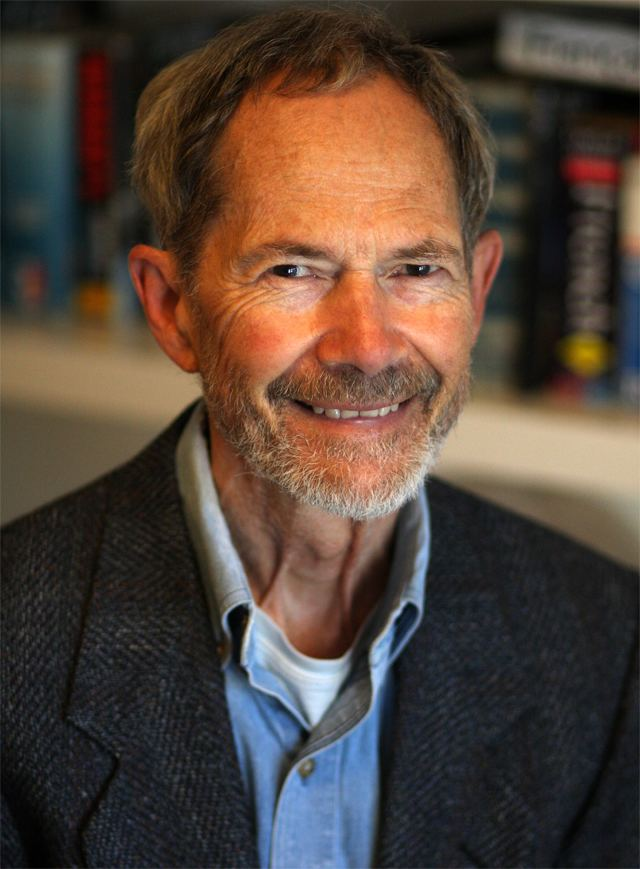
\includegraphics[width=.15\textwidth]{Fred_Glover.jpeg}
	\caption[Fred Glover]{\\Fred Glover}
\end{wrapfloat}


\noindent In fact, the Greek suffix \textit{meta} means “upper level methodology''. 


Metaheuristic algorithms were designed in order to solve problems too difficult for the heuristic algorithms. Hence, metaheuristics provide “acceptable” solutions in a reasonable time for solving hard and complex problems in science and engineering.  This explains the significant growth of interest in metaheuristic domain. Unlike exact optimization
algorithms, metaheuristics do not guarantee the optimality of the obtained solutions~\cite{Talbi_2009}.


There are two types of metaheuristic algorithms:
\begin{description}
	\item[Population based] They can be viewed as an iterative improvement in a population of permutations. At first the population is initialized, then a new one is generated and finally these populations are integrated into a new one using a selection procedure. The search process is stopped when a stopping criterion is satisfied. Some of Population based algorithms are Ant Colony Optimization, Genetic Algorithms, Memetic Algorithms~\cite{Talbi_2009}. 
	\item[Single-solution based] While solving optimization problems, single-solution based metaheuristics improve a single solution. They can be viewed as “walks” through neighborhoods or search trajectories through the search space of the problem. Tabu Search, Simulated Annealing, GRASP, Variable Neighborhood Search belong to this class of metaheuristics~\cite{Talbi_2009}.
\end{description}

\noindent There are three central concepts in metaheuristics:
\begin{description}
	\item[Neighborhood] We define a neighborhood of a feasible solution $\pi \in \Sn$ as a generic function $\mathcal N \colon \pi \to \mathcal P(S_n)$ that maps a solution to a set of solutions.
	\item[Intensification] Exploitation of the best solutions. Often this is achieved by doing a local search starting from the current solution.
	\item[Diversification]  Exploration of the search space, in order to escape from local minimum.
\end{description}

We are going to describe three different metaheuristic algorithms:
\begin{itemize}
	\item Tabu Search. We implemented the original algorithm in~\cite{Skorin_Kapov_1990}.
	\item Ant Colony Optimization. We elaborated a new strategy for the diversification phase with respect to~\cite{Gambardella1999}.
	\item Variable Neighborhood Search. We did not find an implementation of this algorithm for QAP in literature; hence, we devised a new implementation \textit{ex novo}. 
\end{itemize}


\section{Tabu search}
\label{sec:Tabu_search}

\subsubsection{Introduction}


The history of Tabu Search (TS)\index{tabu search} is described in the following table.
\begin{center}
\footnotesize
\begin{tabular}{ll}
\toprule
Year & Event \\
\midrule
1986& Tabu Search algorithm is proposed by Glover~\cite{Glover1986}	\\
1990& Skorin-Kapov implements tabu search for QAP~\cite{Skorin_Kapov_1990}\\
1991& Éric Taillard implements \textit{robust tabu search} for QAP~\cite{Taillard_1991}\\
1994&  Battiti and Tecchiolli~\cite{Battiti_1996} implements \textit{reactive tabu search} for \QAP \\
2011 & Misevicius~\cite{Misevicius2011} implements \textit{iterated tabu search} (ITS) for QAP\\
\bottomrule
\end{tabular}
\end{center}

\noindent In his famous paper of 1986, Fred Glover introduced Tabu\footnote{The name comes from Polynesian word \textit{tàpu} that means prohibited.}  Search algorithm as follows:
\begin{quote}\footnotesize
	From an AI point of view, \textit{tabu search }deviates to an extent from what might be expected of
	intelligent human behavior. Humans are often hypothesized to operate according to some sort of
	random (probabilistic) element which promotes a certain level of “inconsistency”. The resulting
	tendency to deviate from a charted course, sometimes regretted as a source of error, can also prove a
	source of gain. Such a mechanism has been postulated to be useful, even fundamental, to human
	ingenuity.
\end{quote}

\noindent TS is one of the most studied and used algorithm for QAP. In several cases, the methods of this class provide solutions very close to optimality and are among the most effective, if not the best, to tackle the difficult problems at hand. Therefore, these successes have made TS extremely popular~\cite{Gendreau2019}.


\begin{wrapfloat}{figure}{O}{0pt}
	
\includegraphics[width=.15\textwidth]{Jadranka_Skorin_Kapov}
	\caption[Skorin-Kapov]{\\Jadranka Skorin-Kapov}
\end{wrapfloat}


The main idea of TS is to \textit{forbid} certain moves. This is done in order to escape from local optima. To do this, a \textit{tabu list} was adopted. It is an array of size \textit{s} (called \textit{tabu tenure}), that stores the past evolution of the algorithm.

Since there is a rich variety of strategies and tools, there is a lot of freedom in the implementation of a TS.







The first TS algorithm for QAP was presented by  Jadranka Skorin-Kapov, Stony Brook University, New York. Her algorithm starts with an initial permutation $\pi$ and begin an intensification phase using a local search algorithm; she used the neighborhood ${N}_2$, as defined in section~\ref{def:Intorno}. She forbid the $2$-exchange of two units that were swapped during the previous $s$ iterations, inserting them into the tabu list, i.e., every time a $2$-~exchange is performed, the algorithm inserts the two indices swapped into the tabu list. 


After one year, the \textit{robust tabu search} (roTS) was defined by Éric Taillard, École polytechnique fédérale de Lausanne (Lausanne, Switzerland). Based on Skorin-Kapov work, they used the same neighborhood but a different  tabu list. For every facility $i$ and location $j$, the latest iteration at which the facility $i$ occupied location $j$ is recorded. A $2$-exchange $\pi_{i_1i_2}$ is tabu if  both $i_1$ and $i_2$ are assigned to locations they had occupied in the last $s$ iterations. The tabu tenure varies in a cyclic random manner between a lower value $s_\mathrm{min}=\lfloor 0.9 n \rfloor$ and an high value $s_\mathrm{max}=\lceil 1.1n \rceil$. This value is updated every $2 \cdot s_\mathrm{max}$ iterations.

In 1994, Roberto Battiti and Giampietro  Tecchiolli, Instituto Nazionale di Fisica Nucleare (Trento, Italy),  introduced the reactive tabu search (ReTS). They still used neighborhood $N_2$, but the algorithm evolved in a more complex way. In fact, ReTS \textit{reacts} during the evolution of the search by increasing the tabu tenure when a solution is repeated along the search, and decreasing it if no repetition occurs for a certain number of iterations . They used hashing functions, binary trees, bucket lists as tool to store the solution and to check if a neighbour solution was already visited~\cite{Burkard2012}. The numerical results show that ReTS is competitive with ro-TS in terms of number of iterations performed to reach the best known solution~\cite{Burkard2012}.



In 2011, Alfonsas Misevicius  , Kaunas University of Technology, (Kaunas, Lithuania) implemented~\cite{Misevicius2011} \textit{iterated tabu search} (ITS). He combined the roTS with a special type of mutation. As regards tabu tenure, he differentiated from  Taillard's approach. The tabu tenure $s$ various $s$ in a deterministic way: each time it reached a value $s_\mathrm{max}$, it drops to a lower value $s_\mathrm{min}$. For small size problems ($n\le 50$) he used $s_\mathrm{min}=\lfloor 0.2n \rfloor$ and $s_\mathrm{max}=\lceil 0.4n\rceil$. For larger problems ($n>50$) he used $s_\mathrm{min}=\lfloor 0.1n \rfloor$ and $s_\mathrm{max}=\lceil 0.2n\rceil$.

Now we are going to describe the algorithm in details.

\subsubsection{Description of the algorithm} 

In our implementation, we followed the main idea of Skorin-Kapov's work.

We consider two types of memories:\textit{short-term memory}
 and \textit{long-term memory}.
\begin{description}
	\item[Short-term memory ] This memory consists of a tabu list with tabu tenure $s$. This list is used to prevent revisiting previously visited solutions. This is done in order to achieve diversification.
	
	\item[Long-term memory] This memory stores information on the visited solutions during the search. The idea of long-term memory is to record the frequency with which each movement has been realized since the beginning of the algorithm. In our implementation, long-term memory provide an intensification phase.
\end{description}


An other important ingredient is the \textit{aspiration criterion}. It is essentially a condition that, if holds, allows tabu solutions to be accepted. The most common criterion is  to accepts the tabu moves that generate solutions  better than the best one found so far.


Pseudo code~\ref{Pseudocode: Tabu Search} sketches the idea of the algorithm.

The short-term memory is an array of size $s$ where the best local moves performed are stored. Every time that an improvement of the objective function by a $2$-exchange occurs, the move performed is stored in the tabu list, hence it is prohibited. Since the dimension of  list  is finite, when the list is full the next move will replace the oldest one (this is why it forms the short-term memory: it records only the $s$ previous moves). 
 
  We implemented long-term memory as an $n \times n$ matrix $\bm M =(m_{ij})$. Each entry of $\bm M$ is related to the quality of the $2$-exchange done, e.g., if the $2$-exchange $\{1,2\} \to \{2,1\}$  improves the current solution, then we store this information on $\bm M$, updating the matrix as follows:
  \[M_{12} \gets M_{12}+1 \quad  \text{and} \quad  M_{21}\gets M_{21}+1.\]
  
   



\begin{description}
	\item[Input] Tabu tenure $s$, penalty parameter $\mu$, maximum time $t_\mathrm{max}$.
	\item[Output] The obtained solution $p_\mathrm{best}$ and its objective function value $z_\mathrm{best}$.
\end{description}


\begin{algorithm}
	\footnotesize	
	\KwIn{$n$, $\bm F$, $\bm D$, $\mu$, $s$,  $t_\mathrm{max}$}
	\KwOut{$p_\mathrm{best}$, $z_\mathrm{best}$}	
	\tcc{initialization}
	Build an initial solution $p$ with objective function  $z_p=z(p)$ by \texttt{Greedy3} algorithm\;
	$z_\mathrm{best} \gets z_p$\;
	$ p_\mathrm{best} \gets \bm p$\;
	$\bm M \gets \bm 0$\;
	$\tilde{\bm D} \gets \bm D$\;
	\tcc{main loop}
	Call \texttt{CPU\_TIME}  $t$\;
	\While{$t < t_\mathrm{max} $}
	{\label{alglinea:dmin}
		\tcc{improvement of the current solution}
			$d_\text{min} \gets 0$\;
			Starting from $p$, search an admissible local $2$-optimum $p_\mathrm{temp}\in {N}_2(p)$ with objective function value $z_\mathrm{temp}$. This is obtained by a $2$-exchange of indices $(j_1,j_2)$\;
			$d_\mathrm{min} \gets \Delta(p;j_1,j_2)$\;
			\tcc{update short-term memory}
			Add the pair $(j_1,j_2)$ to tabu list\;
			
			
			\If{$d_\mathrm{min} < 0$ }{
				$z_p \gets z_\mathrm{temp}$\;
				$p \gets p_\mathrm{temp}$\;
				\tcc{update long-term memory}
				$m_{j_1j_2}  = m_{j_1j_2}  +1$\;
				$m_{j_2j_1}  = m_{j_2j_1}  +1$\;
				\If{$z_p<z_\mathrm{best}$}{
					$z_\mathrm{best} \gets z_p$\;
					$p_\mathrm{best} \gets p$\;
				}
				Call \texttt{CPU\_TIME}  $t$\;
				Go to~\ref{alglinea:dmin}\;
			}
			\tcc{create a new solution using long-term memory}
			$\tilde{\bm D} \gets  \tilde{\bm D} + \mu \bm M $ \;
			Use \texttt{Greedy3} with matrices $\bm F$ and $\tilde{\bm D}$ to create a new permutation $p$ with objective function $z_p$\;
			Call \texttt{CPU\_TIME} $t$\;
		}
		\caption{Tabu search}
		\label{Pseudocode: Tabu Search}
	\end{algorithm}


\subsubsection{Initialization}%\mbox{}\\


At first algorithm builds an initial permutation. In our implementation it is provided by the by \texttt{Greedy3} method (line 1). The output permutation and its objective function provided by \texttt{Greedy3}  are denoted by $p$ and $z_p$.
 
 The long-term matrix is initialized as the null matrix (line 4).
 A copy of distance matrix $\bm D$ is stored in matrix $\tilde{\bm D}$ (line 5).

\subsubsection{Improvement of the current solution}


The algorithm looks for an improvement of the current solution (lines 9-10). This is done in our implementation by a modified version of \texttt{2optBest} algorithm. 



The difference with \texttt{2optBest} algorithm is that not every move is allowed. At each step, TS controls if the current indices $i_1$ and $i_2$ belong to tabu-list. If this is the case, \texttt{2optBest} variant skips to the next pair of indices.

It is possible to overcome the tabu restriction for a pair $(j_1,j_2)$ if the $2$-exchange $\{j_1,j_2\}\to \{j_2,j_1\}$ improves the best solution  obtained by far $p_\mathrm{best}$.  

The term $d_\mathrm{min}$ is stored (line 10). It is the best improvement of the objective function value obtained.

If $d_\mathrm{min}=0$, this means that the best $2$-exchange found does not improve the current solution. Therefore, $p_\mathrm{temp}$ is an admissible local optimum. The term \textit{admissible} means that it does not belong to the tabu list, or it belongs but provides an improvement of the best permutation found so far $p_\mathrm{best}$.

On the other hand, if $d_\mathrm{min}<0$, then there is indeed an improvement of the objective function value.
Suppose that $\{j_1,j_2\}\to \{j_2,j_1\}$ is the best  admissible $2$-exchange. Then, the $2$-exchange is applied and its objective function value is updated (lines 13-14).

Moreover, if the permutation after the $2$-exchange is the best found so far, the algorithms update $p_\mathrm{best}$ and $z_\mathrm{best}$ (lines 18-20).


This procedure repeats until the actual permutation $p$ cannot be improved any more ($d_\mathrm{min}\ge 0$).


\subsubsection{Updating of the memories}

The short-term memory is updated: the two indices $j_1$ and $j_2$ enter in the tabu list (line 11).

If the tabu list is full, it starts again by substituting the first two index of the list with $j_1$ and $j_2$.
This idea was taken from Skorin-Kapov~\cite{Skorin_Kapov_1990}.

As regards long-term memory, the matrix $\bm M$  is updated by increasing  $m_{j_1,j_2}$ and $m_{j_2,j_1}$ by $1$ (lines 15-16). This memory, unlike tabu list, is never reset its value. Therefore, the indices $j_1$ and $j_2$ remain in $\bm M$ until the end of the algorithm. 

\subsubsection{Creation of a new permutation}

 At this point  the matrix $\tilde{\bm D}$ is updated as $\tilde{\bm D} \gets \tilde{\bm D}+ \mu \bm M$ where $\mu$ is an input penalty parameter (line 24).
 
In our runs, we set 
   
   \begin{equation}
   	\label{eq:ParametroMu}\mu = k \cdot \frac{1}{n^2} \sum_{j=1}^n\sum_{i=1}^n d_{ij}.
   	\end{equation}
   
   \noindent This allow us to adapt the magnitude of $\mu \bm M$  to the one of matrix $\bm D$; 
 
  If $\mu > 0$, the algorithms increases distance between locations frequently swapped, therefore tries to achieve diversification. 
 
 On the other hand, if $\mu < 0$, then distance between locations frequently swapped decreases, hence the algorithm stimulates frequent moves to be chosen.
 


Finally, a constructive algorithm is used to create another solution $p^*$ from the updated matrix $\bm D$. Here the algorithm starts again, setting $p\gets p^*$. 

Note that the only \texttt{Greedy3} algorithm uses the updated matrix $\tilde{\bm D}$, the rest of the algorithm still uses the original distance matrix $\bm D$.



\subsection*{Implementation and parameters calibration}
We implemented algorithm~\ref{Pseudocode: Tabu Search} in Fortran language. The code can be found on \href{https://github.com/TDS-Firenze/QAP/blob/master/TABU_SEARCH.f90}{GitHub}~\cite{Mazzoli2020}.

Since the dimension of the instances are very different, we are going to do two separate calibrations: one for small dimensions ($n < 50$) and an other one for large dimensions ($n \ge 50$).

The algorithm stops whenever the execution time exceeds the input value $t_\mathrm{max}$. We chose $t_\mathrm{max}=\SI{30}{\second}$ for $n<50$ and $t_\mathrm{max}=\SI{60}{\second}$ for $n\ge 50$.

Finally, we run the code on a   i$7$-$9750$H processor with \SI{2.60}{\giga\Hz} clock frequency.

The parameters we have to calibrate are 
\begin{itemize}
	\item the parameter $k$ used in~\eqref{eq:ParametroMu}; 
	\item the size of tabu list $s$; if its value is too small, cycling may occur in the
	search process while if its value is too large, appealing moves may be forbidden and leading to	the exploration of lower quality solutions, producing a larger number of iterations to find the solution desired.
\end{itemize}


To calibrate them, we vary the parameters in a  reasonable range and then we took the values providing best objective function values at average. Like the previous chapter,  we evaluated the Percent Deviation (PD) from the optimal solution.

After some tests we found that the bests values of $k$ were between $-1$ and $-2$, hence we explored it more deeply. Finally, the range of tested parameter values  is 
\begin{itemize}
	\item $k \in \{1, -1,-1.2, -1.4, -1.6, -1.8, -2, -5, -10, -20 \}$
	\item $s \in \{8,10,15,20,25,50,100,200\} $
\end{itemize}



The following pages contain tables where we highlighted in \colorbox{green!40}{green} the optimal solution (or the best known solution) and  in \colorbox{blue!30}{blue} good solutions, even if they were not the optimal.


\subsubsection{Small dimension}
Instances used to calibrate are 
\begin{description}
	\item[\texttt{Tai12a}] We achieved the optimum for several $(k,s)$ (table~\ref{TS:Tai12a})
	. In  most of the cases, the percent error of the solution is less than $4\%$.
	\item[\texttt{Chr20c}] We achieved the optimum for $s = 20,50$ and $k = -1.8$ (table~\ref{TS:chr20c})
	. Other good result were obtained  for  $s = 150$ and $k = -1.8, -2, -5, -10, -20$.
	\item[\texttt{Nug30}] The best solution we achieve (Table~\ref{TS:Nug30}) 
	has a percent error of  $0.03\%$  with $k = -5, -10, -20$ and $s = 20$. All other solutions are pretty good, since they always are under $2\%$ of percent error, except for $k = 1$.
\end{description}




\subsubsection{Large dimension}
We used the following instances:



\begin{description}
	\item[\texttt{Lipa60b}] As we can see in table~\ref{TS:Lipa60b} 
we reached the optimal solution $7$ times: for $\mu = -1$ and $s= 25$, $ 50$, $100$, $150$, for  $\mu = -1.2$ and $s = 8$ and finally for $s = 150$ and $\mu = -1.8$. The instance is asymmetric.
	\item[\texttt{Wil100}]The optimal solution is not known. Every solutions we found has less than $1\%$ of error from the best known solution (which is $64$).
	\item[\texttt{Esc128}] As we can see in table~\ref{TS:Esc128}, 
	We reached the optimum many times. Notice that TS provides optimal solution for every $s$ if $k=-1.8$,$-2$,$-5$,$-10$.

\end{description}

\subsubsection{Conclusions}
%As we can see 
The choice of $k=1$ did not perform well in any instance. This reflects the fact that, for our TS algorithm, intensification is a better strategy than diversification.

For small dimension, we decided to choose $s=20$ and $k=-1.8$, since it provides the optimal solution for \texttt{Chr20c} and for \texttt{Tai12a} and \texttt{Nug30} the sum of the error is minimal: only $2.9\%$.


For large dimension, we chose $s=20$ and $k = -1.4$, since it provides the optimal solution for \texttt{Lipa60b} and \texttt{Esc128}, while only an error of $0.48\%$ for \texttt{Wil100}.


\begin{table}%[p]
	\scriptsize
	\centering
	\begin{tabular}{l*{10}{S[table-format =2.2]}}
		\toprule
		$s$ & \multicolumn{10}c{{$k$}} \\
		\cmidrule{2-11} 
		&    1  &    -1  &  -1.2  &    -1.4    &    -1.6  & -1.8  &    -2  &-5  &
		 -10  &-20    \\
		\midrule
		$8 $  & 6.38 & \best 0 &\best 0 & \best 0 & \best 0 & \best 0 & \best 0 & 3.84  &  3.84 & 3.84\\
		$10$  & 6.30 & \colorbox{green!40}{$0$} & \colorbox{green!40}{$0$} & \colorbox{green!40}{$0$} & \best 0 & \best 0 & \best 0 &  2.08 & \colorbox{green!40}{$0$}& \colorbox{green!40}{$0$}\\
		$15 $ & 6.30 &\colorbox{green!40}{$0$} & \best 0 & \best 0 & \best 0 & \best 0  & \colorbox{green!40}{$0$} & \colorbox{green!40}{$0$} & \colorbox{green!40}{$0$}& \colorbox{green!40}{$0$}\\
		$20$  & 6.30  & \best 0 & \best 0 & \best 0 & 2.80 & 2.80  &2.08   & 2.08 &2.08  &2.08 \\	
		$25$  & 6.30  & 2.80 & 2.80 & 2.08 & \best 0 & 2.08 &  \best 0  & \best 0  & \best 0  &\best 0  \\
		$50$ & 6.30  & 3.84 & 3.84 & 2.80 & 2.80 & 2.08 & 3.84 & \best 0   & \best 0  &\best 0 \\
		$100$ & 6.30  & \best 0  & 2.08 & 2.08 & 2.08 & 2.08 & \best 0   & 2.08 &2.08  &2.08 \\
		$150$ & 6.30  & 6.89 & 6.89 & 2.08 & 2.08 & 2.08 & \best 0  & \best 0 &2.80  &2.80 \\
		\bottomrule
	\end{tabular}
	\caption{Tabu Search for  \texttt{Tai12a}}
	\label{TS:Tai12a}
\end{table}

\begin{table}
	\scriptsize
	\centering
	\begin{tabular}{l*{10}{S[table-format =2.2]}}
	\toprule
	$s$ & \multicolumn{10}c{{$k$}} \\
	\cmidrule{2-11} 
		&    1  &    -1  &  -1.2  &    -1.4    &    -1.6  & -1.8  &    -2  &-5  & -10  &-20    \\
	\midrule
		$8$   & 41.61 & 6.82  & 20.11 & 6.04 & 18.92 & 13.75 &13.75 & 13.75 & 13.75 & 13.75  \\
		$10$  & 41.61 & 21.67 & \colorbox{blue!30}{$4.72$} & 18.22 & 15.90 & 19.37 & 19.37 & 19.37 & 19.37 & 19.37  \\
		$15$  & 39.57 & 20.72 & 18.58 & 11.51 & 24.62 & 18.98 & 18.98 & 18.98 & 18.98 & 18.98  \\
		$20$  & 39.57 & 18.88 & 20.18 & 19.30 & \colorbox{blue!30}{$4.72$} & \best 0 &  19.37 & 19.37 & 19.37 & 19.37  \\
		$25$  & 39.57 & 18.53 & 19.81 & 22.43 & 19.37 & 20.80 & 20.80 & 20.80 & 20.80 & 20.80  \\
		$50$  & 39.57 & 13.75 & 15.90 & 15.20 & 16.69 & \best 0 & 28.72 & 28.72 & 28.72 & 28.72  \\
		$100$ & 36.22 & 17.83 & 18.82 & 18.22 & 18.53 & 20.80 & 20.61 & 20.61 & 20.61 & 20.61  \\
		$150$ & 36.22  & 26.79 & 18.89 & 18.22 & 16.39 & \colorbox{blue!30}{$4.74$}  & \colorbox{blue!30}{$4.74$} & \colorbox{blue!30}{$4.72$}  & \colorbox{blue!30}{$4.72$}  & \colorbox{blue!30}{$4.72$} \\
		\bottomrule
	\end{tabular}
	\caption{Tabu Search for  \texttt{Chr20c}}
	\label{TS:chr20c}
\end{table}

\begin{table}
	\footnotesize
	\centering
	\begin{tabular}{l*{10}{S[table-format =2.2]}}
		\toprule
		$s$ & \multicolumn{10}c{$k$} \\
		\cmidrule{2-11} 
		&    1  &    -1  &  -1.2  &    -1.4    &    -1.6  & -1.8  &    -2  & -5  &
		-10  &-20    \\
		\midrule
		$8$   & 2.45 & 0.98 & 1.27 & 0.78 & 1.44 & 0.95 & 0.95 & 1.96 & 1.96 & 1.96  \\
		$10$  & 2.45 & 1.08 & 0.36 & 0.78 & 1.40 & 1.67 &  1.67 & 1.24 & 1.24 & 1.24  \\
		$15$   & 2.45 & 0.69 & 1.08 & 0.98 & 0.49 & 0.88 & 0.88 & 1.34 & 1.34 & 1.34  \\
		$20$  & 2.45 & 0.85 & 0.88 & 1.47 & 1.47 & 0.82 & 1.86 & \colorbox{blue!30}{$0.10$}  & \colorbox{blue!30}{$0.10$} & \colorbox{blue!30}{$0.10$}  \\
		$25$  & 2.45 & 0.95 & 0.98 & 0.59 & 1.24 & 0.69 & 0.91 & 0.88 & 0.88 & 0.88  \\
		$50$  & 2.45 & 1.05 & 0.62 & 1.14 & 0.46 & 0.75 & 0.69 & 1.01 & 1.01 & 1.01  \\
		$100$ & 2.02 & 0.85 & 0.98 & 0.52 & 1.27 & 1.11 & 1.18 & 0.52 & 0.52 & 0.52  \\
		$150$ & 2.45 & 1.08 & 1.27 & 1.24 & 0.69 & 1.21 & 1.08 & 0.95 & 0.95 & 0.95  \\
		\bottomrule
	\end{tabular}
	\caption{Tabu Search for \texttt{Nug30}}
	\label{TS:Nug30}
\end{table}


\begin{table}
\scriptsize
	\centering
	\begin{tabular}{l*{10}{S[table-format =2.2]}}
		\toprule
		$s$ & \multicolumn{10}c{$k$} \\
		\cmidrule{2-11} 
		&    1  &    -1  &  -1.2  &    -1.4    &    -1.6  & -1.8  &    -2  & -5  &-10  &-20    \\
		\midrule
		$8$  &  19.90 & 19.13    & \best 0 & 19.03   & 19.15 & 19.05   & 19.05 & 19.05 & 19.05 & 19.05    \\
		$10$ &  19.90 & 19.19    & 18.92   & 18.82   & 18.91 & 19.02   & 19.02 & 19.02 & 19.02 & 19.02    \\
		$15$ &  19.54 & 19.09    & 18.90   & 19.44   & 18.92 & 19.11   & 18.92 & 18.92 & 18.92 & 18.92    \\
		$20$ &  19.90 & 19.09    & 19.03   & \best 0 & 18.89 & 19.14   & 19.21 & 18.89 & 18.89 & 18.89    \\
		$25$ &  19.90 & \best 0  & 18.90   & 19.44   & 18.92 & 19.11   & 18.92 & 18.92 & 18.92 & 18.92    \\
		$50$ &  19.90 & \best 0  & 19.14   & 18.86   & 18.90 & 19.03   & 19.03 & 19.03 & 19.03 & 19.03   \\
		$100$&  19.83 & \best 0  & 19.00   & 19.06   & 19.03 & 19.08   & 19.03 & 19.08 & 19.08 & 19.08   \\
		$150$&  19.58 & \best 0  & 18.87   & 19.10   & 19.04 & \best 0   & 19.042 & 19.04 & 19.04 & 19.04   \\
		\bottomrule
	\end{tabular}
	\caption{Tabu Search for  \texttt{Lipa60b}}
	\label{TS:Lipa60b}
\end{table}

\begin{table}
\scriptsize
	\centering
	\begin{tabular}{l*{10}{S[table-format =2.2]}}
		\toprule
		$s$ & \multicolumn{10}c{$k$} \\
		\cmidrule{2-11} 
		&    1  &    -1  &  -1.2  &    -1.4    &    -1.6  & -1.8  &    -2  & -5  &-10  &-20    \\
		\midrule
		$8$   & 0.69 & 0.60 & 0.69 & 0.54 & 0.65 & 0.75 & 0.75 & 0.47 & 0.47 & 0.47 \\
		$10$  & 0.68 & 0.60 & 0.69 & 0.64 & 0.65 & 0.77 & 0.63 & 0.47 & 0.47 & 0.47 \\
		$15$  & 0.73 & 0.60 & 0.72 & 0.60 & 0.65 & 0.82 & 0.65 & 0.59 & 0.59 & 0.59 \\
		$20$  & 0.83 & 0.60 & 0.72 & 0.48 & 0.65 & 0.67 & 0.71 & 0.79 & 0.79 & 0.79 \\
		$30$  & 0.87 & 0.60 & 0.74 & 0.62 & 0.58 & 0.69 & 0.66 & 0.72 & 0.72 & 0.72 \\
		$50$  & 0.67 & 0.60 & 0.74 & 0.62 & 0.58 & 0.69 & 0.66 & 0.72 & 0.72 & 0.72 \\
		$100$ & 0.59 & 0.60 & 0.62 & 0.54 & 0.65 & 0.60 & 0.68 & 0.55 & 0.55 & 0.55 \\
		$150$ & 0.66 & 0.60 & 0.70 & 0.65 & 0.58 & 0.64 & 0.69 & 0.69 & 0.69 & 0.69 \\
		\bottomrule
	\end{tabular}
	\caption{Tabu Search for \texttt{Wil100}}
	\label{TS:Wil100}
\end{table}

\begin{table}
\scriptsize	
\centering
	\begin{tabular}{l*{10}{S[table-format =2.2]}}
		\toprule
		$s$ & \multicolumn{10}c{$k$} \\
		\cmidrule{2-11} 
		&    1  &    -1  &  -1.2  &    -1.4    &    -1.6  & -1.8  &    -2  & -5  &-10  &-20    \\
		\midrule
		$8$ &9.38 & 3.31 & 3.13 & 3.13 & \best 0 &  \best 0 & \best 0 & \best 0 & \best 0 & \best 0  \\
		$10$& 9.38 & 3.13 & \best 0 & \best 0 & \best 0 & \best 0 & \best 0 & \best 0 & \best 0 & \best 0 \\
		$15$& 9.38 & 3.13 & \best 0 & \best 0 & \best 0 & \best 0 & \best 0 & \best 0 & \best 0 & \best 0\\
		$20$& 9.38 & 3.13 & \best 0 & \best 0 & \best 0 & \best 0 & \best 0 & \best 0 & \best 0 & \best 0 \\
		$25$&  9.38 & 3.13 & \best 0 & \best 0 & \best 0 & \best 0 & \best 0 & \best 0 & \best 0 & \best 0 \\
		$50$ & 9.38 & 3.13 & \best 0 & \best 0 & \best 0 & \best 0 & \best 0 & \best 0 & \best 0 & \best 0 \\
		$100$& 9.38 & 3.13 & \best 0 & \best 0 & \best 0 & \best 0 & \best 0 & \best 0 & \best 0 & \best 0 \\
		$150$& 9.38 & 3.13 & 3.13 & 3.13& 9.38 & \best 0 & \best 0 & \best 0 & \best 0 & \best 0\\
		\bottomrule
	\end{tabular}
	\caption{Tabu Search for \texttt{Esc128}}
	\label{TS:Esc128}
\end{table}




\newpage
\afterpage{\clearpage}
\section{Ant Colony Optimization}
\label{sec:Ant_Colony_Optimization}

Ant Colony Optimization algorithm (ACO) was initiated by Dorigo  in 1991. The principle of this method is based on the way Argentine ants \textit{Iridomyrmex humilis} search for food and find their way back to the nest~\cite{Goss1989}. At first, ants explore the area surrounding their nest at random. Then, during the return trip, ants leave a pheromone trail on the ground, in order to guide other ants toward the source of food. The quantity of pheromone left depends on the amount of food found. Pheromone trail evaporates if no one pass there any more.


This algorithm is population based. Hence, at first $m$ initial solutions (the ants) are generated. Then, it comes intensification: each ant is improved in a local search phase. Finally, before the start of the next iteration, the pheromone trail is updated reflecting the \virgolette{experience} of the ants.

\subsection{Hybrid Ant System}


Inspired by Gambardella, Taillard and Dorigo~\cite{Gambardella1999} we implemented a variant of ACO known as Hybrid Ant System (HAS). Nevertheless, we will still refer to this algorithm as ACO.

In this implementation the pheromone trail is a $n \times n$ matrix $\bm T=(\tau_{ij})$, where the entry $\tau_{ij}$ measures how good is assigning facility $i$ to location $j$.
Pseudo code~\ref{Pseudocode : ACO} outlines main steps of ACO.
\begin{algorithm}
	\KwIn{$n$, $\bm F$, $\bm D$, $t_\mathrm{max}$}
	\KwOut{$p_\mathrm{best}$, $z_\mathrm{best}$}
	\caption{ACO algorithm}
	\label{Pseudocode : ACO}
Initialize pheromone trail matrix $\bm T$\;

\While{$t < t_\mathrm{max}$}{
Generate $m$ random initial permutation $\pi^1,\dots,\pi^m$\;
Improve $\pi^1,\dots,\pi^m$ with \texttt{2optFirst} algorithm\;
Let $\pi_\mathrm{best}$ be the best permutation among $\pi^1,\dots,\pi^m$\;
\tcc{solution manipulation}
\For{$k=1,\dots,m$} 
    {Apply $R$  $2$-exchanges to $\pi^k$ to obtain $\hat\pi^k$\;
     Apply \texttt{2optFirst} to $\hat\pi^k$ to obtain $\tilde{\pi}^k$\;
\tcc{intensification}
\eIf{intensification is active}
{$\pi^k\gets $ best permutation between $\pi^k$ and $\tilde{\pi}^k$\;}
{$\pi^k \gets \tilde{\pi}^k$}
}
Deactivate intensification\;
\If{exists $k$ such that $z(\pi^k)< z_\mathrm{best}$}{
Update $\pi_\mathrm{best}$\;
Activate intensification\;}
\tcc{pheromone trail updating}
Update pheromone trail matrix $\bm T$\;
\tcc{diversification}
\If{$S$ loops have been performed without improving $\pi_\mathrm{best}$}{Perform a diversification: $\bm T \gets \bm 0$\;}
}
\end{algorithm}

\subsection{Implementation}

\subsubsection{Pheromone trail initialization}


In the original algorithm by Gambardella et al~\cite{Gambardella1999}, pheromone trail matrix $\bm T$ was initialized by setting every component to the same value $\tau_0=\frac{1}{100 z_\mathrm{best}}$, where $z_\mathrm{best}$ is the best know value of the objective function. 

Instead, we tried another approach: two matrices $\bm M_1$ and $\bm M_2$ are used and then combined to form matrix $\bm T$. 

First, the two matrices $\bm M_1$ and $\bm M_2$ are initialized to $0$. 

Then, $n$ initial permutations are built, by setting
\[
\pi_i= [i,i+1,\dots,n,1,2,\dots,i-1] \qquad \forall i\in{1,\dots,n}
\]
After that, for every permutation $\pi_i$,  \texttt{2optBest} algorithm is applied with the following remarks:
\begin{itemize}
	\item Every $2$-exchange made (hence, every improvement of the solution) is stored: if indices $p$ and $q$  of $\pi_i$ are swapped, therefore  we update the matrix $\bm M_2$ as follows:
	\begin{align*}
	M_2(p,\pi_i(p)) &\gets 	M_2(p,\pi_i(p)) -1, &\quad  M_2(q,\pi_i(q)) &\gets 	M_2(q,\pi_i(q)) -1,\\
	M_2(p,\pi_i(q)) &\gets 	M_2(p,\pi_i(q)) +1, &\quad  M_2(q,\pi_i(p)) &\gets 	M_2(q,\pi_i(p)) +1.
	\end{align*} 
	Finally, since we want $\bm M_2$ to be positive, we set $\bm M_2 \gets \bm M_2 + \min(\bm M_2)$.
	\item At the end of  local search procedure, a final permutation $\tilde{\pi}_i$ is found. Thus, $\bm M_1$ is updated as follows:
	\[
	M_1(r,\tilde{\pi}_i(r)) \gets 	M_1(r,\tilde{\pi}_i(r))+1 \quad \forall r \in \{1,\dots,n\}.
	\]
\end{itemize}

\noindent Finally, pheromone trail matrix $\bm T$ is built summing $\bm M_1$ and $\bm M_2$: \[ \bm T \gets \bm M_1 + \bm M_2.\]
In a nutshell, $\tau_{ij}$ tells us how good is the assignment $\pi(i)=j$. 
\subsubsection{Initialization of solutions}


As in~\cite{Gambardella1999}, $m$ random permutations are chosen. Each permutation is optimized using a local search procedure. Gambardella~\cite{Gambardella1999} used a variant of first improvement algorithm. Instead, we used our \texttt{2optFirst} algorithm.

\subsubsection{Manipulation of solutions}


In~\cite{Gambardella1999}, a number of $R$ $2$-exchanges are applied to each permutation $\pi^k$. These operations provides $m$ new permutations $\hat{\pi}^1,\dots, \hat \pi ^m$. We followed the same procedure. These $R$ swaps are performed as follows:


First, an index $r$ is chosen, randomly between $1$ and $n$.

Then, a second index $s \neq r$ is chosen and the elements $\pi^k_r$ and $\pi^k_s$ are swapped in the current solution $\pi^k$.

The second index $s$ is chosen according to following policy:
\begin{itemize}
	\item With probability given by a parameter $q$, $s$ is chosen such that $\tau_{r\pi_s}+\tau_{s \pi_r}$ is maximum. This means that $s$ is the best $2$-exchange for $r$ we can do, according to pheromone trail matrix $\bm T$.
	\item With probability $(1-q)$, $s$ is chosen with a probability proportional to the values contained in $\bm T$. More precisely, $s$ is chosen with probability
	\begin{equation}
	\label{eq:ACOdensity}
	\frac{\tau_{r\pi_s}+\tau_{s \pi_r}}{\sum_{j \neq r}\left(\tau_{r\pi_j}+\tau_{j \pi_r}\right)}.
	\end{equation}
\end{itemize}
Note that setting $M_2\ge 0$ allows $\tau_{ij}$ to be positive. Therefore,  expression~\eqref{eq:ACOdensity} is indeed a density of probability.  

After the $2$-exchange, \texttt{2optfirst} algorithm is applied to every permutation $\hat{\pi}^k$, obtaining $m$ $2$-optima: $\tilde{\pi}^1\dots, \tilde{\pi}^m$.

\subsubsection{Intensification}

The intensification mechanism is activated when the best solution produced so far $\pi_\mathrm{best}$  has been improved. Intensification remains active while at least one solutions is improved during an iteration. Therefore:
\begin{itemize}
	\item If intensification is active, then each permutation starts its next iteration as the best permutation between $\pi^k$ and $\tilde{\pi}^k$.
	\item If intensification is not active, then the permutation is maintained as~$\tilde{\pi}^k$.
\end{itemize}

\subsubsection{Pheromone trail update}
Pheromone trail is updated by taking into account only the best solution~$\pi_\mathrm{best}$. 

Firstly, the pheromone trail $\bm T$ is weakened by setting $\tau_{ij}= (1-\alpha)\cdot \tau_{ij}$ where $0<\alpha<1$ is a parameter that controls \textit{evaporation} of the trail. A value of $\alpha$ close to $0$ implies that pheromone is more persistent, while a value close to $1$ implies high degree of evaporation (thus, a shorter memory of the system).

Secondly, $\bm T$ is reinforced by considering the best permutation obtained so far $\pi_\mathrm{best}$. 
In~\cite{Gambardella1999}, authors update the pheromone trail $\bm T$ as follows: 
\begin{equation}
\tau_{i\pi_\mathrm{best}(i)} \gets \tau_{i \pi_\mathrm{best}(i)} + \frac{\beta}{z_\mathrm{best}} \qquad \forall i \in \{1,\dots,n\}.
\end{equation}
Instead, we followed an other approach: The algorithm builds matrices $\bm M_1$ and $\bm M_2$ in the same way of pheromone trail initialization, but only considering $\pi_\mathrm{best}$ instead of all the $m$ permutations.

 Finally, we update $\bm T$ as follows:
 
  \begin{equation}\bm T  \gets\bm T  + \left(\bm M_1 + \bm M_2 \right).
\end{equation}

\subsubsection{Diversification}
Diversification mechanism is activated if, during the last $S$ loops, no improvement to the best generated solution is detected.
Diversification consists in erasing all the information contained in the pheromone trail and in randomly generating other $m$ solutions (line 22).

\subsubsection{Complexity}
The complexity of the algorithm can be evaluated as follows: most time consuming part of the algorithm is the local search procedure, which has a computational cost of $O(n^3)$ operations. This is repeated $Im$ times, where $I$ is the number of loops performed. Hence, the total cost of ACO is $O\left(Imn^3\right)$.

\subsection{Parameters calibration}
Table~\ref{tab:ACOParam} shows us the parameters that must be calibrated, the tested ranges and the chosen values.

\begin{table}[htp]
	\small
	\centering
	\caption{Parameters of ACO algorithm}
	\label{tab:ACOParam}
	\begin{tabular}{lccl}
		\toprule
		Name & Symbol & Value & Range tested \\
		\midrule
		Probability & $q$ & $0.85$ &$\{0.15, 0.50, 0.85\}$ \\
		Number of $2$-exchanges performed & $R$& $2$ &$\{5,10,15\}$\\
		Evaporation & $\alpha$ & $0.25$ & $\{0.15, 0.25\}$\\
		Maximum number of non improving loops & $S$&  $5n$ & $\{n, 2n, 5n\}$\\
		Number of ants & $m$ & $10$  & $\{5,10,20\} $\\
		
		
		\bottomrule
	\end{tabular}
\end{table}


We tested various values of each parameters for $6$ instances: \texttt{tai12a}, \texttt{chr20c}, \texttt{nug30}, \texttt{lipa60b}, \texttt{wil100} and \texttt{esc128}.

In this case, we did not make any distinctions between small and large dimensions instances, since no substantially differences were found.




We chose a number of ants $m$ equal to $10$, to limit the computation time required for the algorithm. 

The parameter $S$ was set equal to $5n$. For $S \le n$, the algorithm provides poorly solution with high percentage deviation, even for small dimension instances.

As regards the other parameters, they were experimentally found  to be good and robust for the instance tested, providing an output permutation with less than $1\%$ of PD. 



\newpage

\section{Variable neighborhood Search}
\label{sec:Variable_neighborhood_Search}

\subsubsection{Introduction}


\noindent The Variable Neighborhood Search algorithm (VNS) was introduced by Pierre Hansen and Nenad Mladenovic in 1997~\cite{Mladenovic1997} for the Traveling Salesman Problem (TSP). The literature of VNS for QAP is not as extended as for Tabu Search or Ant Colony Optimization. 

The main idea of the algorithm is to use several neighborhood structures and, when a local optimum is found, to move from one to another.

Now, we present some essential definitions and facts about neighborhood structures. More detail can be found in~\cite[Ch. 3]{Gendreau2019}.

Let us start with two definitions.

\begin{defi}[Neighborhood structure]
	A function $\mathcal N \colon \Sn \to \mathcal P(\Sn)$ that maps  a feasible solution $\pi \in \Sn$ to a set of a solutions $\mathcal N(\pi) \subseteq \Sn$ is called a \textit{neighborhood  structure}.
\end{defi}

\begin{defi}[Local optimum]
	A solution $\pi^*$ is called a \textit{local optimum} with respect to the neighborhood structure $\mathcal N$ if there is no feasible solution $\sigma \in \mathcal N(\pi^*)$ such that $z(\sigma) \le z(\pi^*)$.
\end{defi}
Essentially, we can consider  $\mathcal N(\pi)$ as a set of permutations \textit{close} to $\pi$.

Therefore, the operator $\mathcal N$ allows us to obtain new feasible solutions realizing a determined operation on an initial solution.

Note that neighborhoods $N_r$ defined by~\eqref{def:Intorno} are an example of neighborhood structures, since they map a permutation $\pi$ into the set of permutations that can be reached by $\pi$ by a $r$-exchange.

\subsection{Local search}

\subsubsection{Description of the algorithm}

This procedure is a generalization of the local search algorithms discussed in section~\ref{sec:LocalSearch}. 

Pseudo code~\ref{Pseudocode:LocalSearch} shows the local search algorithm. 


\begin{algorithm}\footnotesize
	\KwIn{An initial permutation $s_1$, a neighborhood structure $\mathcal N$}
	\KwOut{A local optimum $s^*$ w.r.t. $\mathcal N$}
	\Repeat{a local optimum  $s^*$ is found}{
		Examine $\mathcal N(s_1)$\;
		\eIf(){exists $s_2\in \mathcal N(s_1)$ such that $z(s_2)\le z(s_1)$}{
			$s_1 \gets s_2$\;}
		{$s^*\gets s_1$\;
		Exit\;}
	}
	\caption{Local search procedure.}
	\label{Pseudocode:LocalSearch}
\end{algorithm}


Imagine to fix a neighborhood structure $\mathcal N$, with an initial permutation~$s_1$.

Then, the local search starts, and the algorithm exhaustively examines every permutation in $\mathcal N(s_1)$ (line 4).

After investigating $\mathcal N(s_1)$, there are two possibilities:
\begin{enumerate}
	\item A permutation $s_2$ such that $z(s_2)<z(s_1)$ is found.
	\item No better permutation is found. Therefore,  $s_1$ is a local optimum in $\mathcal N_1$, i.e.,  $z(s_1)=\min\left\{z(p) \mid p \in \mathcal N(s_1)\right\}$.
\end{enumerate}

In the first case, the algorithm repeats setting $s_1 \gets s_2$. In the second case, the algorithm stops (lines 4-8).

Since the number of permutations is finite, in a finite number of steps the algorithm provides a local optimum with respect to the neighborhood structure $\mathcal N$ (line 9).

Note that in Section~\ref{sec:LocalSearch}, the neighborhood structure $\mathcal N$ of local search algorithm was $N_r$, for $r=2$ or $r=3$.



Figure~\ref{fig:Local Search} sketches an idea of the local search procedure. The pink oval represents the neighborhoods structure. The local search starts from $s_1$, looks for a \virgolette{better} solution on $\mathcal N(s_1)$ and finds $s_2$. Then, it continues until arriving at $s_5$, which is a local optimum w.r.t. $\mathcal N$. Thus, it stops.

 


\begin{figure}
	\centering
	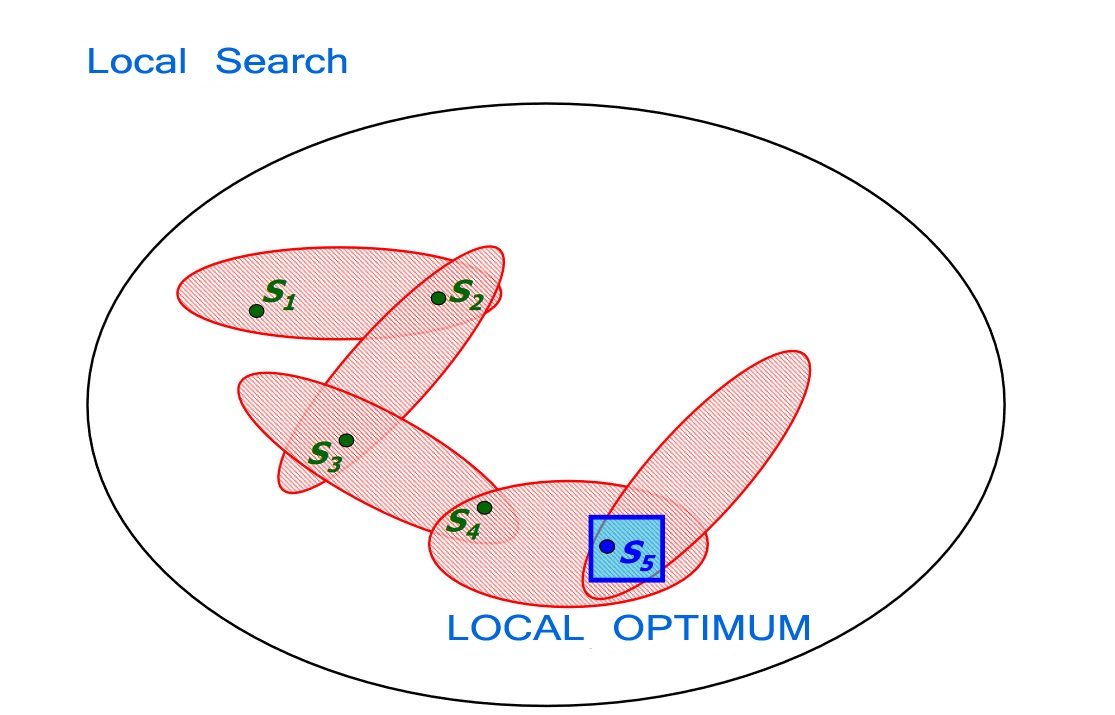
\includegraphics[width=.65\textwidth]{Local_Search.png}
	\caption[Local search procedure]{Local search procedure, starting from initial point $s_1$.}
	\label{fig:Local Search}
\end{figure}

Two final remarks:
\begin{itemize}
	\item The algorithm stops when it finds a local optimum. 
	\item The search is limited to only one neighborhood structure. 
\end{itemize}

The first point suggests us that local search procedure should be used as a part of an intensification method, combined with other technique to escape from local optima.
 
As regards the second point, the algorithm that solves this problem is the Variable neighborhood Search (VNS).

\subsection{Variable neighborhood Search }


The basic idea  of Variable Neighborhood Search algorithm (VNS) is  a  systematic change of neighborhood both within a descent phase to find a local optimum and in a perturbation phase to get out of the corresponding valley~\cite[Ch. 3]{Gendreau2019}.



Suppose we have $\left\{\mathcal N_1,\mathcal N_2, \dots, \mathcal N_k \right\}$, a finite set of pre-selected $k$ neighborhood structures.

Hence, every time a local optimum is reached, the algorithm changes the neighborhood structure and searches a local optimum belonging to the new neighborhood. Once it is reached, VNS  starts again from the beginning, with the first neighborhood structure. 


\begin{figure}
	\centering
	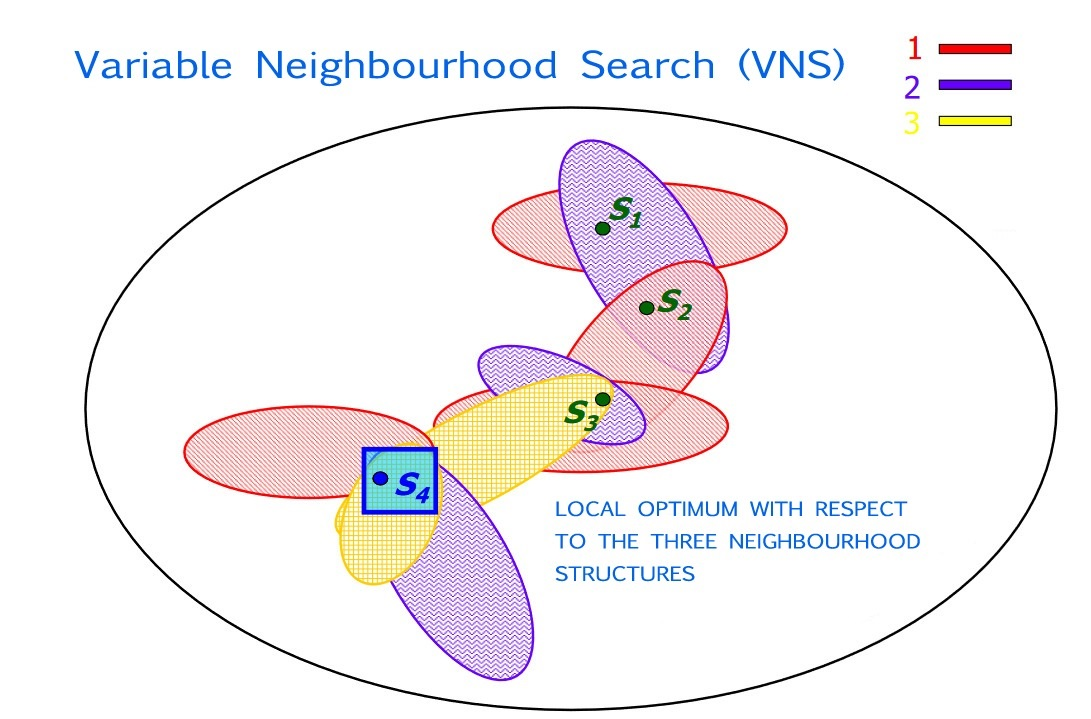
\includegraphics[width=.65\textwidth]{VNS.jpg}
	\caption{VNS procedure}
	\label{fig:VNS}
\end{figure}


Figure~\ref{fig:VNS} shows us a VNS procedure with three different neighborhood structures. The algorithm starts with $s_1$ and explores the first neighborhood (in red). If $s_1$ is a local optimum w.r.t. $\mathcal N_1$, then it explores $\mathcal{N}_2(s_1)$ and finds $s_2$. Now, it starts again looking for a local optimum w.r.t. $\mathcal{N}_1(s_2)$ and so on. The algorithm stops as soon as he finds a local optimum w.r.t. all the three neighborhood structures.



VNS algorithm is based on three simple facts~\cite{Gendreau2019}:
\begin{description}
	\item[Fact 1] A local minimum with respect to one neighborhood structure is not necessarily so for another.
	\item[Fact 2] A global minimum is a local minimum with respect to all possible neighborhood structures.
	\item[Fact 3] For many problems, local minima with respect to one or several $\mathcal N_j$ are relatively close to each other. 
\end{description}

There are three different ways to use Facts 1-3:
\begin{enumerate}
	\item Deterministic;
	\item Stochastic. 
	\item Both deterministic and stochastic. 
\end{enumerate} 

In Section~\ref{sec:VND} we will focus on  \textit{Variable neighborhood Descent} (VND) , an algorithm which belongs to the first approach. 

In Section~\ref{sec:GVNS} we will study the \textit{General Variable Neighborhood Search} (GVNS), an example of the third approach.


\subsection{Variable Neighborhood Descent}
\label{sec:VND}

The Variable neighborhood Descent algorithm (VND) performs a change of neighborhoods in a deterministic way. As the name says, it is a descent method, hence it could be implemented as an intensification phase of more sophisticated algorithm.

Pseudo code~\ref{Pseudocode: VND} describes a general VND method.

\begin{algorithm}
	\KwIn{$s$, $\left\{\mathcal N_1,\dots, \mathcal N_{k_\mathrm{max}}\right\}$\;}
	\KwOut{$s^*$, a local optimum w.r.t. all neighborhood structures}
	$k\gets 1$\;
	\While{$k\le k_\mathrm{max}$}{
		Do a local search in  $\mathcal N_k(s)$; a local optimum $\tilde{s}$ w.r.t. $\mathcal N_k$ is found\;
		\eIf(){$z(\tilde{s})<z(s)$}{
			$s \gets \tilde{s}$\;
			$k \gets 1$\;}
		{$k \gets k + 1$\;}
	}
$s^* \gets s$\;
	\caption{VND algorithm}
	\label{Pseudocode: VND}
	
\end{algorithm}


\subsubsection{Description of the algorithm}

As  usual, let us suppose we have a set of prefixed neighborhood structures $\left\{\mathcal N_k \mid k=1,\dots, k_\mathrm{max}\right\}$ and an initial permutation $s$.

The algorithm starts doing a local search with respect to the first neighborhood structure $\mathcal N_1$. A local optimum $s'$ w.r.t. $\mathcal N_1$ is found (line 3).

Now there are two cases:
\begin{enumerate}
	\item If $z(s')<z(s)$ then $s'$ is a \textit{better} permutation than $s$, therefore the algorithms starts again exploring $\mathcal N_1(s')$ (lines 5-6).
	\item If $z(s') = z(s)$, then $s'$ is a local optimum with respect to $\mathcal N(s)$, the algorithm explores the next neighborhood structure $\mathcal N_2(s')$ (line 8).
\end{enumerate}

This procedure is repeated until a local optimum w.r.t. all neighborhood structures is found (lines 2-10). Note that $z(s') > z(s)$ cannot occur, since $s'$ is a local optimum with respect to $\mathcal N_k(s)$.

The final solution $s$ is a local optimum with respect to all neighborhood structures (line 11).

\subsubsection{Implementation}

We implemented VND in the most immediate way. We used the neighborhood structures defined in~\ref{def:Intorno}, in particular we used ${N}_2$ and ${N}_3$.

We know that there are two strategies for a local search on these neighborhood: first-improvement and best-improvement. Therefore, we implemented two algorithms: 
\begin{itemize}
	\item  VNDfirst, that uses a first-improvement strategy.
	\item  VNDbest, that uses a best-improvement strategy.	
\end{itemize}

Pseudocode~\ref{Pseudocode: VNDfirst} shows the VNDfirst algorithm. The best-improvement version is totally similar, except for lines $6$ and $9$, where algorithms \texttt{2optBest} and \texttt{3optBest} are called.


\begin{algorithm}
	\KwIn{$n$, $\bm F$, $\bm D$, $\pi_\mathrm{start}$, $z_\mathrm{start}$\;}	
	\KwOut{$\pi_\mathrm{best}$, $z_\mathrm{best}$\;}
$\pi_\mathrm{best} \gets \pi_\mathrm{start}$\;
$z_\mathrm{best} \gets z_\mathrm{start}$\;	
	$k\gets 1$\;
	\While{$k\le 2$}{
		\If{$k = 1$}{Call \texttt{2optFirst}($p_\mathrm{best},z_\mathrm{best},\pi,z_\pi$)}
         \ElseIf   {$k = 2$}{Call \texttt{3optFirst}($p_\mathrm{best},z_\mathrm{best},\pi,z_\pi$)}
         
         \eIf{$z_\pi<z_\mathrm{best}$}{
			$z_\mathrm{best} \gets z_\pi$\;
			$\pi_\mathrm{best} \gets \pi$\;
			$k \gets 1$\;}
		{$k \gets k + 1$\;}
	}
Stop: $\pi_\mathrm{best}$ is $2$-optimal and $3$-optimal\;
	\caption{VNDfirst algorithm}
	\label{Pseudocode: VNDfirst}
	
\end{algorithm}
%\bel{
Note that VND algorithm only achieves intensification, therefore we still lack some procedure for diversification phase. Here it will come the GVNS algorithm.
%}


\subsection{GVNS}
\label{sec:GVNS}
A more general approach is the General Variable neighborhood Search algorithm (GNVS).

\subsubsection{Description of the algorithm}
GVNS introduces a new set of neighborhood structures $ \left\{\mathcal P_1,\dots,\mathcal P_{h_\mathrm{max}}\right\}$. Hence, we have two sets of neighborhood structures:
\begin{itemize}
	\item The set $\left\{\mathcal N_1,\dots,\mathcal N_{k_\mathrm{max}}\right\}$ which will be used in VND algorithm (intensification phase).
	\item The set $ \left\{\mathcal P_1,\dots,\mathcal P_{h_\mathrm{max}}\right\}$ which will be used to move randomly (diversification phase).
\end{itemize}
 In general,  these two sets can be totally  different even in the number of elements ($k_\mathrm{max}\neq h_\mathrm{max}$).

Pseudo code~\ref{Pseudocode: GVNS} conveys an idea of the algorithm.

\begin{algorithm}
	\KwIn{a set of neighborhood structures $\left\{\mathcal N_1,\dots,\mathcal N_{k_\mathrm{max}}\right\}$ for VND algorithm, a set of neighborhood structures $\mathcal \{\mathcal P_1,\dots,\mathcal P_{h_\mathrm{max}} \}$ for diversification phase}
	\KwOut{$s^*$ local optimum w.r.t. $\mathcal N_1, \dots \mathcal N_{k_\mathrm{max}}$}
	Construct an initial solution $s$\;
	\While{stopping criterion}
	{
		$h \gets 1$\; \label{step1GVNS}
		\tcc{diversification}
		Perturbation: choose at random   $s'\in \mathcal P_h(s)$\; \label{step2GVNS}
		\tcc{intensification}
		Realize a VND starting from $s'$, obtaining $s''$\;
		\If{$z(s'') < z(s)$}
		{
			$s \gets s''$\;
			Go to step~\ref{step1GVNS}\;
		}
		\eIf{$h\le h_\mathrm{max}$}
		{ 
			$h \gets h+1$\;
			Go to step~\ref{step2GVNS}\;}
	{Exit}
		
	}
	$s^* \gets s$\;
	$s^*$ is the minimum w.r.t. neighborhood structures $\mathcal N_1,\mathcal N_2,\dots,\mathcal N_{k_\mathrm{max}}$.
	\caption{GVNS pseudo code}
	\label{Pseudocode: GVNS}
	
\end{algorithm}

First, the algorithm builds an initial point $s$ (line 1).

Then, the main loop starts (line 2). At first, a diversification is applied: the initial permutation $s$ is moved in a random way (we will discuss this step in the next section) into another permutation $s'$ belonging to $\mathcal P_1(s)$ (line 4).

After that, in order to achieve intensification, VND algorithm is applied to $s'$ and provides a permutation $s''$ which is local optimum w.r.t. $\mathcal N_1,\dots,\mathcal N_{k_\mathrm{max}} $ (line 5).

Now there are two cases:
\begin{enumerate}
	\item If $z(s'')<z(s)$, then the algorithm starts again with the diversification phase updating permutation $s$ as $s''$ (line 7).
	 \item If $z(s'')\ge z(s)$ , then the neighborhood $\mathcal P_2$ is considered. A perturbation is applied and the permutation $s''$ is randomly moved into another permutation belonging to $\mathcal P_2(s'')$ (lines 10-12).
\end{enumerate}

This procedure is repeated until $h>h_\mathrm{max}$ (line 16). In this case, $s^*$ is a local optimum w.r.t. neighborhood structures $\mathcal N_1,\dots, \mathcal N_{k_\mathrm{max}}$. 

In general, $s^*$ is not an optimum for the other neighborhood structures~$\mathcal P_h$, since their role is just to provide diversification perturbing solution.


The stopping criterion we chose is the execution time $t_\mathrm{max}$ and a maximum number of $\num{10000}$ loops without any improvement. 






Figure~\ref{fig:GVNS} shows GVNS procedure with three neighborhood structures.

	The algorithm starts with an initial permutation $s_1$ (obtained after a diversification phase, which is omitted in the figure for sake of clarity). 
	
Then, a VND is applied and a new permutation $s_2$ is obtained. Then, the diversification phase starts again.

This procedure repeats until the stopping criterion.



\begin{figure}
	\centering
	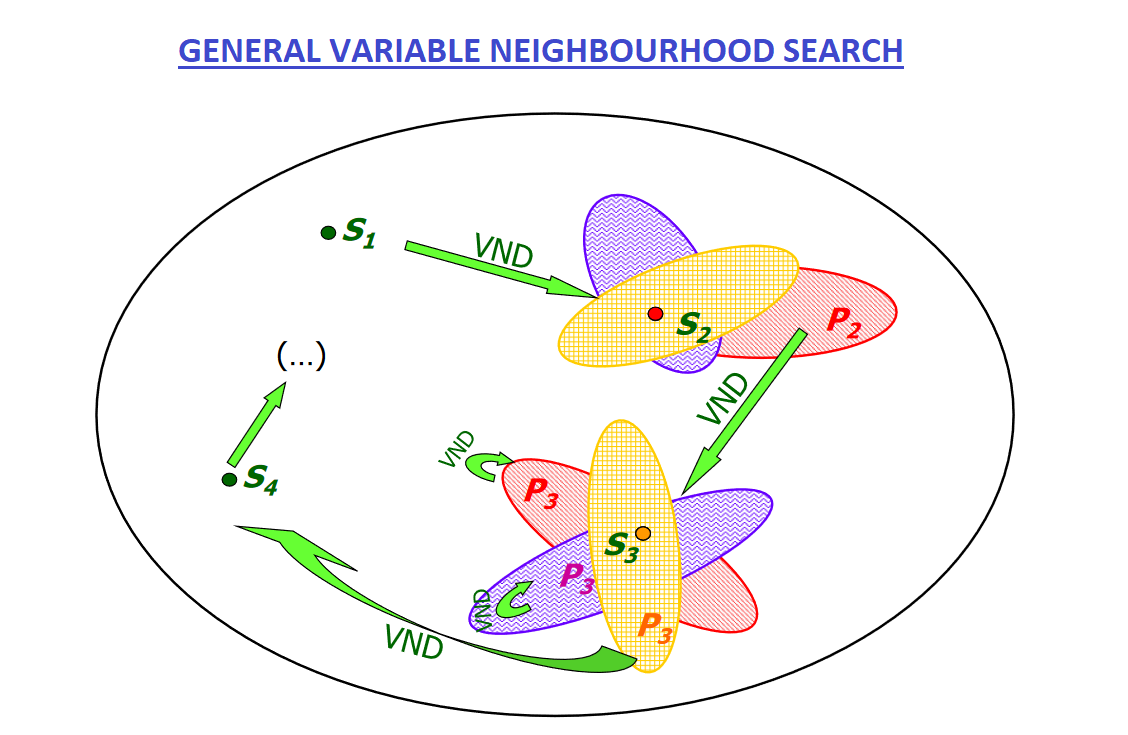
\includegraphics[width=.65\textwidth]{GVNS.png}
	\caption{GVNS procedure.}
	\label{fig:GVNS}
\end{figure}



\subsubsection{Implementation}


For the intensification phase we used VNDfirst and VNDbest algorithms, with neighborhood structures $\left\{ N_2,  N_3\right\}$. Since there are two VND procedures, we implemented two GVNS algorithms: GVNSfirst and GVNSbest.




As regards the GVNS algorithms, we added one extra neighborhood structure: $\left\{ N_2,  N_3, \mathcal P \right\} $, where $ \mathcal P(\pi)$ is the neighborhood (a singleton) formed by dividing the permutation $\pi$ in two and swapping the first part with the second one. 

For example, 
\[
\text{If $\pi = [\colorbox{yellow}{$1$,$4$},\colorbox{red!40}{$3$,$2$}]$, then $ \mathcal P(\pi) =[\colorbox{red!40}{$3$,$2$},\colorbox{yellow}{$1$,$4$}]$}   
\]

Thus, in our case, $k_\mathrm{max}=2$ and $h_\mathrm{max}=3$.

Input and output are the same on every  algorithm:
\begin{description}
	\item[Input]  The initial solution $p$ and $z_p$ is its objective function value.
	\item[Output] The best found solution $p_\mathrm{best}$ and $z_\mathrm{best}$ its objective function value.
\end{description}

As we can see, there are no parameters to calibrate.


Pseudo code~\ref{Pseudocode: GVNSfirst} explains GVNDfirst algorithm. The best-improvement version is the same, exchanging only line 17.

The stopping criterion we chose is the execution time $t_\mathrm{max}$ and a maximum number of $\num{10000}$ loops without any improvement. 


\begin{algorithm}
	\footnotesize
\KwIn{$n$, $\bm F$, $\bm D$, $p$, $z_p$}
\KwOut{$p_\mathrm{best},z_\mathrm{best}$}

\tcc{initialization}
$p_\mathrm{best} \gets p $\;
$z_\mathrm{best} \gets z $\;
%$i \gets 1$ \;
\tcc{main loop}
\Repeat{stopping criterion}{
	$j \gets 1$ \;\label{GVNS:j=1}

\While{$j\le3$}{
		\tcc{diversification}
	\lIf{$j > 3$}{exit}
	\uElseIf{$j =1$}{
	Do a random $2$-exchange $\{i_1,i_2\}$ on $p$\;
    $z_p \gets z_p + \Delta(p;i_1,i_2)$ }
	\uElseIf{$j =2$}{
	Do a random $3$-exchange $\{i_1,i_2,i_3\}$ on $p$\;
	$z_p \gets z_p + \Delta^1(p;i_1,i_2,i_3)$ }
	\ElseIf{$j =3$}{
		Swap the first half of $p$ with the second half, call it again $p$\;
		Evaluate the objective function $z_p$ of $p$\;
	}
\tcc{intensification}
Call VNDfirst algorithm\;
\If{$z(p)<z(p_\mathrm{best})$}{
$p_\mathrm{best} \gets p $\;
$z_\mathrm{best} \gets z $\;
%$it \gets 0$\;
Go to~\ref{GVNS:j=1}
}
$j \gets j + 1 $ \;

	
}	}	
\caption{GVNSfirst}
\label{Pseudocode: GVNSfirst}
\end{algorithm}
